\documentclass[aspectratio=169]{beamer}
\usefonttheme{serif}
\usepackage{xeCJK}
\usepackage{fontspec}
\usepackage{graphicx}
\usepackage{listings}
\usepackage{xcolor}
\usepackage{indentfirst}
\usepackage{tikz}
\usepackage{amssymb}
\usepackage{amsthm}
\usepackage{amsmath}
\usepackage{tabularx}
\usepackage{hyperref}
\usepackage{ulem}
\usepackage{version}
\usepackage{thmtools}
\usepackage{qtree}
\usepackage{algpseudocode}
\usepackage{mathtools}
\usepackage{multicol}
\usepackage{color}
\usepackage{ulem}

% the lstlistings package
\usepackage{listings}
% highlighting lines in listings
\usepackage{linehighlight}

% set colors for code background and highlighting
\definecolor{codehighlight}{rgb}{0.95,0.8,0.8}
\definecolor{codebackground}{rgb}{0.95,0.95,0.95}

\AtBeginDocument{%
    \DeclareSymbolFont{pureletters}{T1}{lmr}{\mddefault}{it}%
}

\XeTeXlinebreaklocale "zh"
\XeTeXlinebreakskip = 0pt plus 1pt

\setCJKmainfont{NotoSansTC-Medium.otf}

\usetikzlibrary{arrows,decorations.markings,decorations.pathreplacing}
\newenvironment{Hint}{\noindent\textbf{Hint.}}{}

\tikzstyle {graph node} = [circle, draw, minimum width=1cm]
\tikzset{edge/.style = {decoration={markings,mark=at position 1 with %
            {\arrow[scale=2,>=stealth]{>}}},postaction={decorate}}}

\lstset{
    basicstyle=\ttfamily\large,
    stepnumber=1,
    numbersep=3pt,
    commentstyle=\color{black!50},
    keywordstyle=\color{white!0!blue},
    stringstyle=\color{black!50!green},
    showspaces=false,
    showstringspaces=false,
    showtabs=false,
    tabsize=4,
    captionpos=b,
    breaklines=true,
    breakatwhitespace=false,
    escapeinside={\%*}{*)},
    morekeywords={*}
}

\AtBeginSection[]{
  \begin{frame}
  \vfill
  \centering
  \begin{beamercolorbox}[sep=8pt,center,shadow=true,rounded=true]{title}
    \usebeamerfont{title}\insertsectionhead\par%
  \end{beamercolorbox}
  \vfill
  \end{frame}
}

\title{動態規劃 (二)}
\author{sam571128}
\date{2022-07-06}

\usetheme{Madrid}
\usecolortheme{default}
\setbeamertemplate{itemize items}[square]
\setbeamertemplate{enumerate items}[default]
\setbeamertemplate{blocks}[default]

\begin{document}

\frame{\titlepage}

\begin{frame}{目錄}
    \begin{itemize}
        \item DP 的概念
        \item $O(n \log n)$ LIS
        \item 各種背包問題
        \item 區間 DP (Range DP)
        \item 位元 DP (Bitmask DP)
        % \item 輪廓線 DP (DP on Broken Profile)
        % \item 數位 DP (Digit DP)
        \item 單調隊列優化 (Monotonic Queue Optimization)
        \item 矩陣快速冪 (Matrix Exponentiation)
        \item 更多例題
    \end{itemize}
\end{frame}

\section{DP 的概念}

\begin{frame}{DP 的性質}
    這堂課,我們要來更加地了解 DP,以下為解決 DP 問題時會用到的一些性質
    \begin{itemize}
        \item 重複子問題 (overlapping subproblems)
        \item 最佳子結構 (optimal substructures)
        \item 狀態的轉移順序會是一張有向無環圖 (DAG)
    \end{itemize}
\end{frame}

\begin{frame}{重複子問題 (overlapping subproblems)}
    \begin{itemize}
        \item<1-> 一個問題,可以被拆分成很多個小問題,而這些小問題在遞迴時,可能會被重複使用到很多次,而非每次皆會產生一個新的問題。
        \item<2-> 例子: 費氏數列 ($f_n = f_{n-1} + f_{n-2}$)
    \end{itemize} \pause
    \begin{center}
        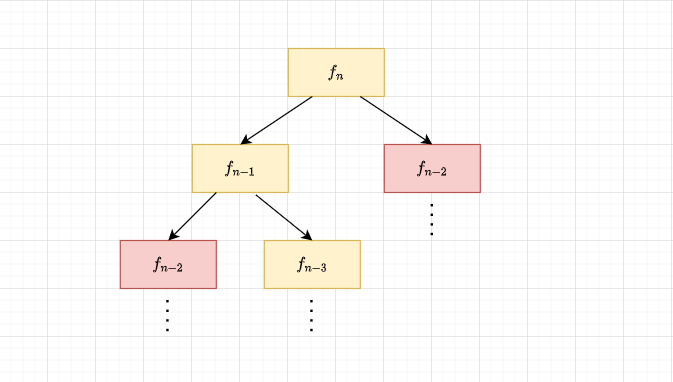
\includegraphics[scale=0.45]{images/overlapping_subproblems.png}
    \end{center}
\end{frame}

\begin{frame}[fragile]{重複子問題 (overlapping subproblems)}
    \begin{itemize}
        \item 一個問題,可以被拆分成很多個小問題,而這些小問題在遞迴時,可能會被重複使用到很多次,而非每次皆會產生一個新的問題。
        \item 例子: 費氏數列 ($f_n = f_{n-1} + f_{n-2}$)
        \item 可以使用動態規劃紀錄狀態,記憶化 (memoization) 就是其中一種例子
        \item 左邊的 code 為 $O(f_n) \approx O(2^n)$,而右邊的 code 為 $O(n)$
    \end{itemize} 
    \begin{multicols}{2}
    \begin{lstlisting}[language=C++,basicstyle=\small]
int f(int x){
    if(x <= 1) 
        return 1;
    else
        return f(x-1) + f(x-2);
}
    \end{lstlisting}
    \begin{lstlisting}[language=C++,basicstyle=\small]
int f(int x){
    if(dp[x]) return dp[x];
    if(x <= 1) 
        return dp[x] = 1;
    return dp[x] = f(x-1) + f(x-2);
}
    \end{lstlisting}
    \end{multicols}
\end{frame}

\begin{frame}{最佳子結構 (optimal substructures)}
    \begin{itemize}
        \item<1-> 對於某個狀態的最佳解,可以從小狀態的最佳解轉移過來
        \item<2-> DP 的轉移式通常會有 $dp[i]$ 表示前 $i$ 個 $\ldots$ 的最佳解 
        \item<2-> 而轉移式也通常以類似的方式去思考並且轉移而來
        \item<3-> 題外話:貪心的題目通常也會滿足這個性質
    \end{itemize}
\end{frame}

\begin{frame}{DP 的轉移順序}
    \begin{itemize}
        \item 轉移順序必須是一張 DAG (有向無環圖)
        \item 不能夠發生 $f(b)$ 從 $f(a)$ 轉移,卻又讓 $f(a)$ 從 $f(b)$ 轉移的情形
        \item 下圖為一個線性 DP 可能的轉移順序 
        \begin{center}
            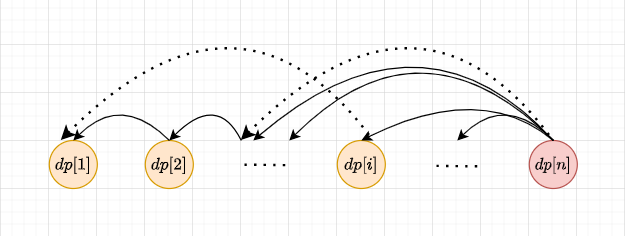
\includegraphics[scale=0.75]{images/DP_DAG.png}
        \end{center}
    \end{itemize}
\end{frame}

\begin{frame}{DP 的轉移順序}
    \begin{itemize}
        \item 轉移順序必須是一張 DAG (有向無環圖)
        \item 不能夠發生 $f(b)$ 從 $f(a)$ 轉移,卻又讓 $f(a)$ 從 $f(b)$ 轉移的情形
        \item 下圖為一個二維 DP 可能的轉移順序
        \begin{center}
            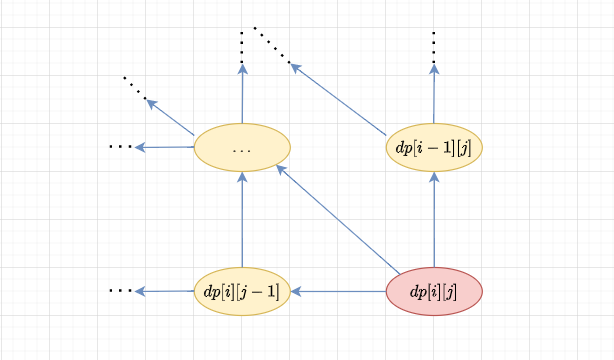
\includegraphics[scale=0.5]{images/DP_DAG_2D.png}
        \end{center}
    \end{itemize}
\end{frame}

\begin{frame}{DP 的轉移順序}
    \begin{itemize}
        \item 轉移順序必須是一張 DAG (有向無環圖)
        \item 不能夠發生 $f(b)$ 從 $f(a)$ 轉移,卻又讓 $f(a)$ 從 $f(b)$ 轉移的情形
        \item 這個概念等一下講到區間 DP (Range DP) 與位元 DP 時,會再次遇到
    \end{itemize}
\end{frame}

\section{Longest Increasing Subsequnce (最長遞增子序列)}

\begin{frame}{Longest Increasing Subsequnce (最長遞增子序列)}
    \begin{block}{最長遞增子序列}
        你有一個 $n$ 項的陣列 $a_1,a_2,\dots,a_n$,請在這個陣列中找到最長遞增子序列的長度 \\
        \vspace{5mm}
        最長遞增子序列: 找到一個集合 $\{p_1,p_2,\dots,p_k\}, \ 1 \le p_i \le n$,使得 $a_{p_1} < a_{p_2} < \dots < a_{p_k}$ 且 $k$ 是最大的。
    \end{block}
    在上一堂課,想必大家都已經學會這題如何在 $O(n^2)$ 的時間解決了!
\end{frame}

\begin{frame}{Longest Increasing Subsequnce (最長遞增子序列)}
    \begin{block}{最長遞增子序列}
        你有一個 $n$ 項的陣列 $a_1,a_2,\dots,a_n$,請在這個陣列中找到最長遞增子序列的長度 \\
        \vspace{5mm}
        最長遞增子序列: 找到一個集合 $\{p_1,p_2,\dots,p_k\}, \ 1 \le p_i \le n$,使得 $a_{p_1} < a_{p_2} < \dots < a_{p_k}$ 且 $k$ 是最大的。
    \end{block}
    假設 $dp[i]$ 為停在第 $i$ 個元素時,最長遞增子序列的長度 \pause \newline
    那麼我們可以枚舉每一個元素 $i$ 以及所有 $j < i$,轉移式為 
    $$dp[i] = \max_{1 \le j < i, \ a_j < a_i}(dp[i], dp[j]+1)$$ \newline \pause
    時間複雜度即為 $O(n^2)$
\end{frame}

\begin{frame}{Longest Increasing Subsequnce (最長遞增子序列)}
    \begin{block}{最長遞增子序列}
        你有一個 $n$ 項的陣列 $a_1,a_2,\dots,a_n$,請在這個陣列中找到最長遞增子序列的長度 \\
        \vspace{5mm}
        最長遞增子序列: 找到一個集合 $\{p_1,p_2,\dots,p_k\}, \ 1 \le p_i \le n$,使得 $a_{p_1} < a_{p_2} < \dots < a_{p_k}$ 且 $k$ 是最大的。
    \end{block}
    事實上,這個題目有 $O(n \log n)$ 的作法,而這兩種分別是
    \begin{enumerate}
        \item 二分搜
        \item 使用資料結構 (BIT、線段樹)
    \end{enumerate}
    而第二種做法,明天會由 Colten 來教各位,我們來談談第一種方式
\end{frame}

\begin{frame}{Longest Increasing Subsequnce (最長遞增子序列)}
    以下為 DP 表格與原本的陣列 \\
    \begin{center}
        \begin{tabular}{|c||c|c|c|c|c|c|c|c|}
        $a_i$   &  1 & 4 & 5 & 3 & 6 & 7 & 5 & 9 \\
        \hline
        $dp[i]$ &  1 & 2 & 3 & 2 & 4 & 5 & 2 & 6
        \end{tabular}
    \end{center} \pause 
    
    設一個 $v$ 陣列,而 $v[j]$ 表示著當 $dp[i]$ 為 $j$ 時,$a_i$ 的最小值
    
    \begin{center}
        \begin{tabular}{|c||c|c|c|c|c|c|c|c|}
        $j$   &  1 & 2 & 3 & 4 & 5 & 6 \\
        \hline
        $v[j]$ &  1 & 3 & 5 & 6 & 7 & 9
        \end{tabular}
    \end{center} \pause 
    會發現 $v$ 會是遞增的,我們可以一邊更新 $v$,一邊二分搜尋找 $dp[i]$ 的答案
\end{frame}

\begin{frame}[fragile]{Longest Increasing Subsequnce (最長遞增子序列)}
    程式碼如下,十分簡單: (複雜度: $O(n \log n)$)
    \vspace{3mm}
    \begin{lstlisting}[language=C++]
int dp[MAXN], arr[MAXN];
vector<int> v;

for(int i = 1;i <= n;i++) {
    int idx = lower_bound(v.begin(), v.end(), arr[i]) - v.begin();
    dp[i] = idx + 1;
    if(idx == v.size()) v.push_back(arr[i]);
    else v[idx] = arr[i];
}

cout << v.size() << "\n";
    \end{lstlisting}
\end{frame}

\begin{frame}{例題}
    \begin{block}{APCS 2021 一月場 p4 - 飛黃騰達}
        有一隻企鵝 Gino 一開始停在座標 $(0,0)$ 的位置,在每一次移動,他只能往上或往右走,而第一象限中,一共有 $n$ 個果實,每個果實的位置在 $(x_i,y_i)$,請問企鵝 Gino 最多可以吃到幾個果實?
    \end{block} \pause
    我們將果實以 $x$ 座標進行排序之後,只要對 $y$ 座標找到 LIS 的長度,就是這題的答案了!
\end{frame}

\begin{frame}{練習題}
    \begin{block}{CSES - Increasing Subsequence}
        請找到給定陣列的最長遞增子序列。
    \end{block}
    \begin{block}{TIOJ 1941 - 直升機抓寶 (Helicopter)}
        由於題目較難解釋,請至 TIOJ 查看
    \end{block}
    \begin{block}{USACO Guide - LCS on Permutations}
        給你兩個 $1 \sim n$ 的排列,請找到這兩個排列的 LCS (最長共同子序列)
    \end{block}
\end{frame}

\section{各種背包問題}

\begin{frame}{背包問題種類}
    \begin{itemize}
        \item $0/1$ 背包問題
        \item 無限背包問題
        \item 有限背包問題
        \item 混合背包問題 (同時出現很多種)
        \item 二維背包問題
        \item 分組背包問題
        \item 分數背包
    \end{itemize}
\end{frame}

\begin{frame}{$0/1$ 背包問題}
    \begin{block}{$0/1$ 背包問題 (CSES - Book Shop)}
        你有一個容量為 $C$ 的背包,有 $n$ 個物品,每個物品的重量為 $w_i$,每個物品可以拿一個或者不拿,請問最多可以拿多少物品?
    \end{block} \pause
    $0/1$ 背包問題的意思是指每個物品都可以拿 $0$ 個或 $1$ 個
\end{frame}

\begin{frame}{$0/1$ 背包問題}
    \begin{block}{$0/1$ 背包問題 (CSES - Book Shop)}
        你有一個容量為 $C$ 的背包,有 $n$ 個物品,每個物品的重量為 $w_i$,每個物品可以拿一個或者不拿,請問最多可以拿多少物品?
    \end{block} 
    這個問題其實跟之前的硬幣問題很像,也就是我們說過貪心不一定成立的那個問題 \\ \pause
    那我們來講講這個問題的作法吧
\end{frame}

\begin{frame}{$0/1$ 背包問題}
    \begin{block}{$0/1$ 背包問題 (CSES - Book Shop)}
        你有一個容量為 $C$ 的背包,有 $n$ 個物品,每個物品的重量為 $w_i$,每個物品可以拿一個或者不拿,請問最多可以拿多少物品?
    \end{block} 
    我們設 $dp[i][j]$ 表示對於前 $i$ 個物品湊出總重量為 $j$ 的時候,最多可以拿幾個物品。 \pause
    接著,我們分別枚舉那 $n$ 個物品,則轉移式會是 
    $$dp[i][j] = \max(dp[i-1][j-w[i]]+1)$$ 
\end{frame}

\begin{frame}[fragile]{$0/1$ 背包問題}
    程式碼大概可以寫成以下的樣子
    \begin{lstlisting}[language=C++]
for(int i = 1;i <= n;i++){
    for(int j = 0;j <= C;j++){
        if(j-w[i] >= 0){
            dp[i][j] = max(dp[i][j], dp[i-1][j-w[i]] + 1);
        }
    }
}
    \end{lstlisting}
\end{frame}

\begin{frame}[fragile]{$0/1$ 背包問題}
    不過,我們可以使用滾動 DP 的技巧,把第一個維度壓掉,時間複雜度: $O(nC)$
    \begin{lstlisting}[language=C++]
for(int i = 1;i <= n;i++){
    for(int j = C;j >= 0;j--){
        if(j-w[i] >= 0){
            dp[j] = max(dp[j], dp[j-w[i]] + 1);
        }
    }
}
    \end{lstlisting}
    注意! 第二個迴圈必須由 $C$ 開始枚舉到 $0$,否則一個物品可能會多拿!
\end{frame}

\begin{frame}{$0/1$ 背包問題}
    題外話: 在演算法中有很多個名稱含有 $0/1$ 的算法,大家要搞清楚每個的分別!
    \begin{center}
        \begin{tabular}{|c|c|}
            \hline 
            演算法名稱 & $0/1$ 的意義 \\ \hline \hline
            $0/1$ 背包問題 & 每個物品只能拿 $1$ 個或 $0$ 個 \\ \hline
            $0/1$ 枚舉 (位元枚舉) & 用二進位的方式進行枚舉 \\ \hline
            $0/1$ 二分搜 (? & 我不知道,據說是 dreamoon 發明的,倍增法二分搜 \\ \hline
            $0/1$ BFS & 圖的邊只有 $0/1$ 時,用 BFS 在 $O(V+E)$ 找到最短路徑 \\ \hline
        \end{tabular}
    \end{center}
\end{frame}

\begin{frame}{無限背包問題}
    \begin{block}{無限背包問題 (Coin Combinations II)}
        你有一個容量為 $C$ 的背包,有 $n$ 個物品,每個物品的重量為 $w_i$,每個物品可以拿任意數量個,請問最多可以拿多少物品?
    \end{block} \pause
    無限背包問題的意思是指每個物品都可以拿任意數量個。
 \end{frame} 
 
\begin{frame}{無限背包問題}
    \begin{block}{無限背包問題 (Coin Combinations II)}
        你有一個容量為 $C$ 的背包,有 $n$ 個物品,每個物品的重量為 $w_i$,每個物品可以拿任意數量個,請問最多可以拿多少物品?
    \end{block} 
    DP 狀態的假設與 $0/1$ 背包十分相似 \\ \pause
    設 $dp[i][j]$ 表示對於前 $i$ 個物品湊出總重量為 $j$ 的時候,最多可以拿幾個物品。 \\ \pause
    接著,我們分別枚舉那 $n$ 個物品,則轉移式會是 
    $$dp[i][j] = \max(dp[i-1][j-w[i]]+1)$$ \pause
    欸? 不是一模一樣嗎?
\end{frame} 

\begin{frame}[fragile]{無限背包問題}
    無限背包問題與 $0/1$ 背包問題的差別只在實作上! 以下是範例 code \\
    \begin{center}
        \begin{lstlisting}[language=C++]
for(int i = 1;i <= n;i++){
    for(int j = 0;j <= C;j++){
        dp[i][j] = dp[i-1][j];
        if(j-w[i] >= 0){
            dp[i][j] = max(dp[i][j], dp[i][j-w[i]] + 1);
        }
    }
}
        \end{lstlisting}
    \end{center}
\end{frame} 

\begin{frame}[fragile]{無限背包問題}
    同樣可以使用滾動 DP 壓掉一個維度,時間複雜度: $O(nC)$
    \begin{center}
        \begin{lstlisting}[language=C++]
for(int i = 1;i <= n;i++){
    for(int j = 0;j <= C;j++){
        if(j-w[i] >= 0){
            dp[j] = max(dp[j], dp[j-w[i]] + 1);
        }
    }
}
        \end{lstlisting}
    \end{center}
\end{frame} 

\begin{frame}[fragile]{有限背包問題}
    \begin{block}{有限背包問題 (CSES - Book Shop II)}
        你有一個容量為 $C$ 的背包,有 $n$ 個物品,每個物品的重量為 $w_i$,每個物品的數量為 $a_i$ 個,請問最多可以拿多少物品?
    \end{block} 
    基本上轉移式跟前兩個也是一模一樣,不過追加了物品數量的限制,我們一樣直接看看實作
\end{frame} 


\begin{frame}[fragile]{有限背包問題}
    有限背包的程式碼 (滾動)
    \begin{center}
        \begin{lstlisting}[language=C++]
for(int i = 1;i <= n;i++){
    for(int x = 1;x <= a[i];x++){
        for(int j = C;j >= 0;j--){
            if(j-w[i] >= 0){
                dp[j] = max(dp[j], dp[j-w[i]] + 1);
            }
        }
    }
}
        \end{lstlisting}
    \end{center}
    有沒有發現什麼?
\end{frame} 

\begin{frame}[fragile]{有限背包問題}
    有限背包的程式碼 (滾動),時間複雜度 $O(\sum_{i=1}^n a_i C)$
    \begin{center}
        \begin{lstlisting}[language=C++]
for(int i = 1;i <= n;i++){
    for(int x = 1;x <= a[i];x++){
        for(int j = C;j >= 0;j--){
            if(j-w[i] >= 0){
                dp[j] = max(dp[j], dp[j-w[i]] + 1);
            }
        }
    }
}
        \end{lstlisting}
    \end{center}
    其實這份 code 就只是我們把 $a_i$ 個物品想成是 $a_i$ 個不同物品,做 $0/1$ 背包 \pause
    但是... 我們真的需要將他拆成那麼多物品嗎? 
\end{frame} 

\begin{frame}[fragile]{有限背包問題 - 物品拆分}
    \begin{itemize}
        \item<1-> 想想看一個概念,組出 $0 \sim n$ 的數字,我們最少需要多少數字呢?
        \item<2-> 真的需要 $n$ 個 $1$ 嗎?
        \item<3-> 二進位!
    \end{itemize}
\end{frame} 

\begin{frame}[fragile]{有限背包問題 - 物品拆分}
    我們可以將 $a_i$ 拆成 $1$、$2$、$4$、$\cdots$、$2^k$ 個、$a_i-(2^{k+1}-1)$ 個 \\
    \vspace{5mm}
    而物品的數量就被我們從原本的 $\sum_{i=1}^n a_i$,變成了 $\sum_{i=1}^n \lg(a_i)$ 了! \\
    時間複雜度: $O(n \lg(\max(a_i)) C)$
\end{frame} 

\begin{frame}[fragile]{有限背包問題 - 還能更快嗎?}
    事實上,有限背包問題還有更快的方式,可以把 $\log$ 給壓掉,不過那個要使用到這堂課後面會教的單調隊列優化。有興趣的可以自己查查看做法。
\end{frame} 

\begin{frame}[fragile]{混合背包問題}
    現在,物品可能有無限多個,一個,或者 $a_i$ 個
    \begin{itemize}
        \item 剛剛有提到無限背包和 $0/1$ 背包的差別在迴圈的順序 
        \item 同時,我們也講到,我們可以藉由物品拆分,將有限背包問題轉成 $0/1$ 背包問題。
        \item 那們我們就在分不同的方式處理,無限背包自己處理,$0/1$ 背包自己處理即可
    \end{itemize}
\end{frame} 

\begin{frame}[fragile]{混合背包問題}
    無限背包用這個 
    \begin{lstlisting}[language=C++]
    for(int j = 0;j <= C;j++){
        if(j-w[i] >= 0){
            dp[j] = max(dp[j], dp[j-w[i]] + 1);
        }
    }
    \end{lstlisting}
    有限背包和 $0/1$ 用這個
    \begin{lstlisting}[language=C++]
    for(int j = C;j >= 0;j--){
        if(j-w[i] >= 0){
            dp[j] = max(dp[j], dp[j-w[i]] + 1);
        }
    }
    \end{lstlisting}
\end{frame} 

\begin{frame}[fragile]{二維背包問題}
    \begin{block}{二維背包問題}
        你有一個可以載重 $M$ 且容量為 $C$ 的背包,有 $n$ 個物品,每個物品的重量為 $w_i$,體積為 $v_i$,每個物品可拿可不拿,請問最多可以拿多少物品?
    \end{block} 
    除了重量以外,多了體積! 要怎麼處理呢? \\ \pause
    狀態多開一維!
\end{frame} 

\begin{frame}[fragile]{二維背包問題}
    \begin{block}{二維背包問題}
        你有一個可以載重 $M$ 且容量為 $C$ 的背包,有 $n$ 個物品,每個物品的重量為 $w_i$,體積為 $v_i$,每個物品可拿可不拿,請問最多可以拿多少物品?
    \end{block} 
    設 $dp[i][j][k]$ 表示總重量為 $j$ 且容量為 $k$ 時,最多可以裝幾個物品。 \\
    \vspace{5mm}
    轉移式為:
        $$dp[i][j][k] = \max(dp[i-1][j-w[i]][k-v[i]]+1)$$
\end{frame} 

\begin{frame}[fragile]{二維背包問題}
    時間複雜度: $O(nMC)$,實作程式碼如下: 
    \begin{lstlisting}
for(int i = 1;i <= n;i++){
    for(int j = M;j >= 0;j--){
        if(j-w[i] >= 0){
            for(int k = C; k >= 0; k--){
                dp[i][j][k] = max(dp[i][j][k], dp[i-1][j-w[i]][k-v[i]] + 1);
            }
        }
    }
}
    \end{lstlisting}
\end{frame} 

\begin{frame}[fragile]{分組背包問題}
    \begin{block}{分組背包問題}
        你有一個容量為 $C$ 的背包,一共有 $t$ 組,每一組有 $a_i$ 個物品,同一組最多只能選一個,請問最多可以拿多少物品?
    \end{block} 
    有沒有人有什麼想法呢?
\end{frame} 

\begin{frame}[fragile]{分組背包問題}
    時間複雜度: $O(nC \sum_{i=1}^t a_i)$,實作程式碼如下: 
    \begin{lstlisting}
for(int i = 1;i <= t;i++){
    for(int j = M;j >= 0;j--){
        if(j-w[i] >= 0){
            for(int k = 0; k <= v[t].size(); k++){
                dp[j] = max(dp[j], dp[j-w[i][k]] + 1);
            }
        }
    }
}
    \end{lstlisting}
\end{frame} 

\begin{frame}[fragile]{分數背包問題}
    \begin{block}{二維背包問題}
        你有一個可以容量為 $C$ 的背包,有 $n$ 個物品,每個物品的重量為 $w_i$,價值為 $v_i$,每個物品你可以拿 $0 \sim 1$ 個 (可以拿一部分),最大可以拿到多少價值?
    \end{block} \pause
    這個其實不是 DP,直接 Greedy 拿取 CP 值 ($\dfrac{v_i}{w_i}$) 最大的即可 
\end{frame} 

\section{區間 DP (Range DP)}

\begin{frame}{區間 DP (Range DP)}
    \begin{block}{AtCoder DP Contest pN - Slimes}
        有 $n$ 隻史萊姆排成一列,而每一次,你可以選擇相鄰的史萊姆,若兩隻史萊姆的大小為 $a,b$,則他們會合併成一個小為 $a+b$ 的史萊姆,並消耗 $a+b$ 的能量。請找到讓這 $n$ 隻史萊姆合併成一隻大史萊姆所需花費的最小能量。
    \end{block} \pause
    這題的想法與之前大家所寫過的不太一樣,他的狀態設計不再只是像以前的 $dp[i]$ 表示前 $i$ 個合併後的最小能量了
\end{frame}

\begin{frame}{區間 DP (Range DP)}
    \begin{block}{AtCoder DP Contest pN - Slimes}
        有 $n$ 隻史萊姆排成一列,而每一次,你可以選擇相鄰的史萊姆,若兩隻史萊姆的大小為 $a,b$,則他們會合併成一個小為 $a+b$ 的史萊姆,並消耗 $a+b$ 的能量。請找到讓這 $n$ 隻史萊姆合併成一隻大史萊姆所需花費的最小能量。
    \end{block} 
    我們假設 $dp[l][r]$ 表示將整個區間 $[l,r]$ 的史萊姆合併之後,所需花費的最小能量。 \pause \\
    而轉移式會是
    $$dp[l][r] = \max_{l \le k < r}(dp[l][k] + dp[k+1][r] + \sum_{i=l}^r a_i)$$
    邊界狀態為 
    $$dp[i][i] = 0$$
\end{frame}

\begin{frame}{區間 DP (Range DP)}
    \begin{block}{AtCoder DP Contest pN - Slimes}
        有 $n$ 隻史萊姆排成一列,而每一次,你可以選擇相鄰的史萊姆,若兩隻史萊姆的大小為 $a,b$,則他們會合併成一個小為 $a+b$ 的史萊姆,並消耗 $a+b$ 的能量。請找到讓這 $n$ 隻史萊姆合併成一隻大史萊姆所需花費的最小能量。
    \end{block} 
    不過這時,有個很重要的問題出現了! 轉移的順序該是如何呢?
\end{frame}

\begin{frame}[fragile]{區間 DP (Range DP)}
    以下有兩種不同的轉移順序,我們來看看何者會是正確的 \\
    \vspace{5mm}
    第一種: 
    \begin{lstlisting}[language=C++]
for (int l = 1; l <= n; l++) {
    for (int r = 1; r <= n; r++) {
        for (int k = l; k <= r; k++) {
            dp[l][r] = max(dp[l][r], dp[l][k] + dp[k+1][r] + sum(l,r));
        }
    }
}       
    \end{lstlisting} 
\end{frame}

\begin{frame}[fragile]{區間 DP (Range DP)}
    以下有兩種不同的轉移順序,我們來看看何者會是正確的 \\
    \vspace{5mm}
    第二種: 
    \begin{lstlisting}[language=C++]
for (int l = n; l >= 1; l--) {
    for (int r = l; r <= n; r++) {
        for (int k = l; k < r; k++) {
            dp[l][r] = max(dp[l][r], dp[l][k] + dp[k+1][r] + sum(l,r));
        }
    }
}       
    \end{lstlisting}
\end{frame}

\begin{frame}[fragile]{區間 DP (Range DP)}
    答案是第二種! \\
    \vspace{5mm}
    \begin{lstlisting}[language=C++]
for (int l = n; l >= 1; l--) {
    for (int r = l; r <= n; r++) {
        for (int k = l; k < r; k++) {
            dp[l][r] = max(dp[l][r], dp[l][k] + dp[k+1][r] + sum(l,r));
        }
    }
}       
    \end{lstlisting}
\end{frame}

\begin{frame}[fragile]{區間 DP (Range DP)}
    \begin{itemize}
        \item 第一種方式在轉移的時候會有很大的問題
        \item 我們可能還沒處理好小狀態,就直接去用小狀態計算大狀態的答案了
        \item 而這是我們不想要看到的
    \end{itemize}
\end{frame}

\begin{frame}[fragile]{區間 DP (Range DP)}
    \begin{block}{AtCoder DP Contest pN - Slimes}
        有 $n$ 隻史萊姆排成一列,而每一次,你可以選擇相鄰的史萊姆,若兩隻史萊姆的大小為 $a,b$,則他們會合併成一個小為 $a+b$ 的史萊姆,並消耗 $a+b$ 的能量。請找到讓這 $n$ 隻史萊姆合併成一隻大史萊姆所需花費的最小能量。
    \end{block} 
    而這題的時間複雜度為 $O(n^3)$ (使用前綴和計算區間和)
\end{frame}

\begin{frame}[fragile]{區間 DP (Range DP)}
    \begin{block}{AtCoder DP Contest pL - Deque}
        Koying 和 Colten 在玩遊戲,他們在地上擺了 $n$ 個石頭排成一列,並在上面用奇異筆寫上了數字。由 Koying 先手,他們每一次可以拿取最前面或最後面的石頭,並得到那顆石頭上面寫下的數字加入各自的分數中。兩個人都以最佳策略進行遊戲,請問最後兩人的分數分別會是多少?
    \end{block} \pause
    有了剛剛那題的經驗之後,這題我們留給大家一點時間進行思考
\end{frame}

\begin{frame}[fragile]{區間 DP (Range DP)}
    \begin{block}{AtCoder DP Contest pL - Deque}
        Koying 和 Colten 在玩遊戲,他們在地上擺了 $n$ 個石頭排成一列,並在上面用奇異筆寫上了數字。由 Koying 先手,他們每一次可以拿取最前面或最後面的石頭,並得到那顆石頭上面寫下的數字加入各自的分數中。兩個人都以最佳策略進行遊戲,請問最後兩人的分數分別會是多少?
    \end{block} 
    假設 $dp[l][r]$ 為\textbf{先手}在區間 $[l,r]$ 時,能夠獲得的最大分數 \pause \\
    轉移式為
    $$dp[l][r] = \max(a_l + sum(l,r) - dp[l+1][r], sum(l,r) - dp[l][r-1] + a_r)$$ \pause 
    邊界狀態為
    $$dp[i][i] = a_i$$
\end{frame}

\begin{frame}[fragile]{區間 DP (Range DP)}
    \begin{block}{Codeforces 607B - Zuma}
        給你一個 $n$ 項的陣列 $a_1, a_2, \dots, a_n$,你每次可以刪除一個回文子陣列,請問最少要刪除幾次,才能將整個陣列消除。
    \end{block} \pause
    同樣留給大家一點時間想想看
\end{frame}

\begin{frame}[fragile]{區間 DP (Range DP)}
    \begin{block}{Codeforces 607B - Zuma}
        給你一個 $n$ 項的陣列 $a_1, a_2, \dots, a_n$,你每次可以刪除一個回文子陣列,請問最少要刪除幾次,才能將整個陣列消除。
    \end{block} 
    這題的想法與前兩題差不多,假設 $dp[l][r]$ 為將 $[l,r]$ 消完所需的最少次數。 \\
    不過轉移式有兩種 case
\end{frame}

\begin{frame}[fragile]{區間 DP (Range DP)}
    Case 1: $a_l = a_k$,轉移 $dp[l+1][k-1]+dp[k+1][r]$
    \begin{center}
        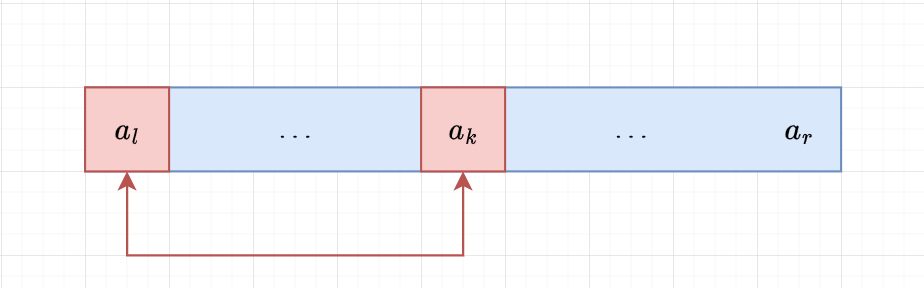
\includegraphics[scale=0.3]{images/Zuma_1.png}
    \end{center} \pause
    Case 2: 消除 $a_l$,轉移 $1+dp[l+1][r]$
    \begin{center}
        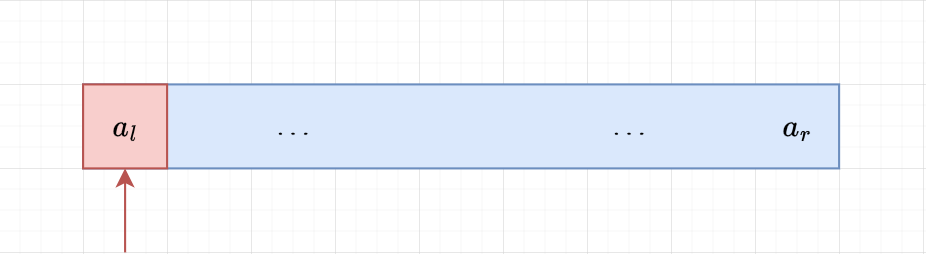
\includegraphics[scale=0.3]{images/Zuma_2.png}
    \end{center} 
\end{frame}

\begin{frame}[fragile]{練習}
    Case 1: $a_l = a_k$,轉移 $dp[l+1][k-1]+dp[k+1][r]$
    \begin{center}
        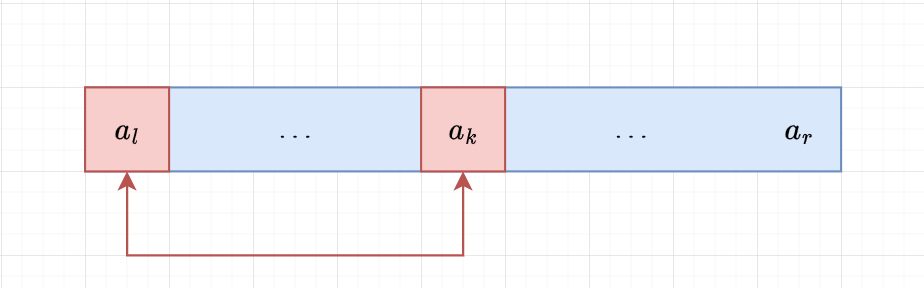
\includegraphics[scale=0.3]{images/Zuma_1.png}
    \end{center} \pause
    Case 2: 消除 $a_l$,轉移 $1+dp[l+1][r]$
    \begin{center}
        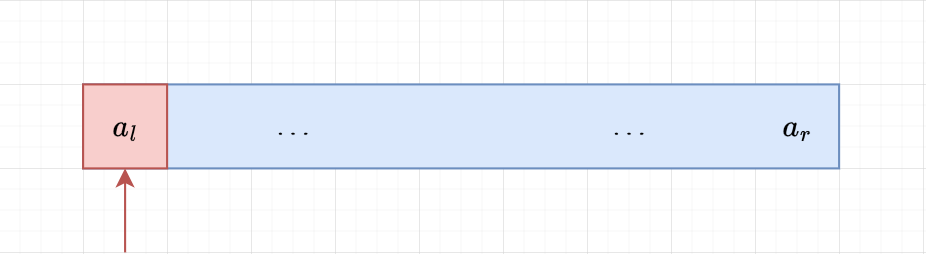
\includegraphics[scale=0.3]{images/Zuma_2.png}
    \end{center} 
\end{frame}

\section{位元 DP (Bitmask DP)}

\begin{frame}[fragile]{位元 DP (Bitmask DP)}
    \item 在我們看位元 DP 之前,先幫大家複習一下位元運算 \\
    \begin{center}
        \begin{tabular}{|c|c|}
            \hline
             名稱 & 符號 \\ \hline \hline
             and  & $\mathtt{\&}$ \\ \hline
             or   & $\mathtt{|}$  \\ \hline
             xor  & $\mathtt{\^}$ \\ \hline
             left shift & $\mathtt{<<}$ \\ \hline
             right shift & $\mathtt{>>}$ \\ \hline
        \end{tabular}
    \end{center}
\end{frame}

\begin{frame}[fragile]{位元 DP (Bitmask DP)}
    \begin{block}{旅行推銷員問題 (Travelling Salesman Problem)}
        在某個國家,一共有 $n$ 個城市,以及兩個城市之間的距離,現在有一個旅行推銷員,他希望從城市 $1$ 開始出發,恰好經過所有城市一次之後,再回到城市 $1$。請問他最少要走過多少距離? \\
        \vspace{5mm}
        測資範圍: $1 \le n \le 20$
    \end{block}
\end{frame}

\begin{frame}[fragile]{位元 DP (Bitmask DP)}
    \begin{block}{旅行推銷員問題 (Travelling Salesman Problem)}
        在某個國家,一共有 $n$ 個城市,以及兩個城市之間的距離,現在有一個旅行推銷員,他希望從城市 $1$ 開始出發,恰好經過所有城市一次之後,再回到城市 $1$。請問他最少要走過多少距離?\\
        \vspace{5mm}
        測資範圍: $1 \le n \le 20$
    \end{block} 
    \begin{center}
        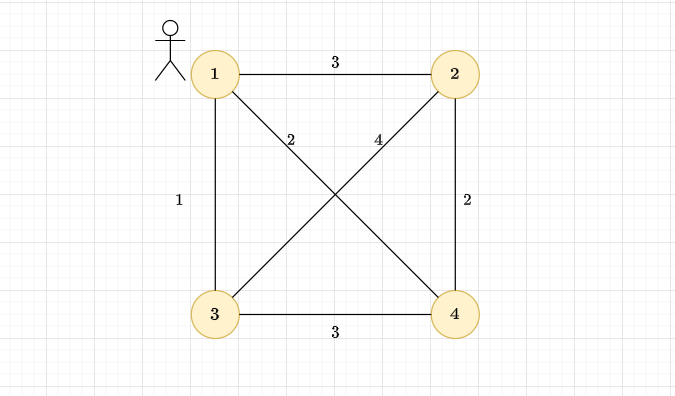
\includegraphics[scale=0.4]{images/TSP.png}
    \end{center}
\end{frame}

\begin{frame}[fragile]{位元 DP (Bitmask DP)}
    \begin{block}{旅行推銷員問題 (Travelling Salesman Problem)}
        在某個國家,一共有 $n$ 個城市,以及兩個城市之間的距離,現在有一個旅行推銷員,他希望從城市 $1$ 開始出發,恰好經過所有城市一次之後,再回到城市 $1$。請問他最少要走過多少距離?\\
        \vspace{5mm}
        測資範圍: $1 \le n \le 20$
    \end{block} 
    \begin{center}
        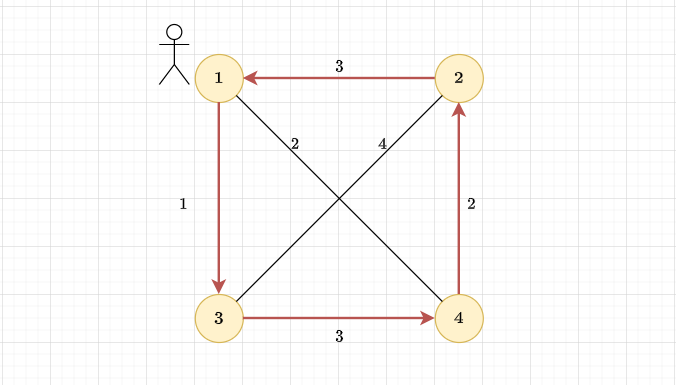
\includegraphics[scale=0.4]{images/TSP2.png}
    \end{center}
\end{frame}

\begin{frame}[fragile]{位元 DP (Bitmask DP)}
    \begin{block}{旅行推銷員問題 (Travelling Salesman Problem)}
        在某個國家,一共有 $n$ 個城市,以及兩個城市之間的距離,現在有一個旅行推銷員,他希望從城市 $1$ 開始出發,恰好經過所有城市一次之後,再回到城市 $1$。請問他最少要走過多少距離?\\
        \vspace{5mm}
        測資範圍: $1 \le n \le 20$
    \end{block} 
    \begin{center}
        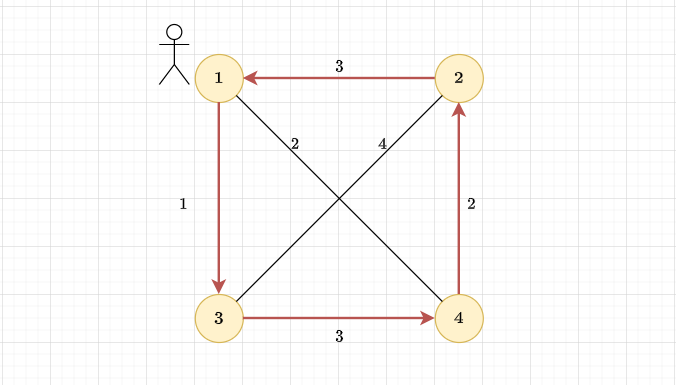
\includegraphics[scale=0.4]{images/TSP2.png}
    \end{center}
\end{frame}

\begin{frame}[fragile]{位元 DP (Bitmask DP)}
    \begin{block}{旅行推銷員問題 (Travelling Salesman Problem)}
        在某個國家,一共有 $n$ 個城市,以及兩個城市之間的距離,現在有一個旅行推銷員,他希望從城市 $1$ 開始出發,恰好經過所有城市一次之後,再回到城市 $1$。請問他最少要走過多少距離?\\
        \vspace{5mm}
        測資範圍: $1 \le n \le 20$
    \end{block} 
    這題的 DP 狀態的設計與大家之前看過的應該都不太一樣,因此我們直接來看看作法吧!
\end{frame}

\begin{frame}[fragile]{位元 DP (Bitmask DP)}
    \begin{block}{旅行推銷員問題 (Travelling Salesman Problem)}
        在某個國家,一共有 $n$ 個城市,以及兩個城市之間的距離,現在有一個旅行推銷員,他希望從城市 $1$ 開始出發,恰好經過所有城市一次之後,再回到城市 $1$。請問他最少要走過多少距離?\\
        \vspace{5mm}
        測資範圍: $1 \le n \le 20$
    \end{block} 
    我們假設 $dp[i][mask]$ 為停在第 $i$ 個城市,$mask$ 表示已經經過了幾個城市的最短距離。 \\ \pause
    範例: $dp[1][0011]$ 表示停在第 $1$ 個城市,已經走過了第 $0$ 和 $1$ 個城市
\end{frame}

\begin{frame}[fragile]{位元 DP (Bitmask DP)}
    \begin{block}{旅行推銷員問題 (Travelling Salesman Problem)}
        在某個國家,一共有 $n$ 個城市,以及兩個城市之間的距離,現在有一個旅行推銷員,他希望從城市 $1$ 開始出發,恰好經過所有城市一次之後,再回到城市 $1$。請問他最少要走過多少距離?\\
        \vspace{5mm}
        測資範圍: $1 \le n \le 20$
    \end{block} 
    轉移式的話:
        $$dp[i][mask] = \max_{j \in adj[i]}(dp[j][mask\^2^i] + dis[j][i])$$ \pause \\
    時間複雜度: $O(n 2^n)$
\end{frame}

\begin{frame}[fragile]{位元 DP (Bitmask DP)}
    \begin{block}{旅行推銷員問題 (Travelling Salesman Problem)}
        在某個國家,一共有 $n$ 個城市,以及兩個城市之間的距離,現在有一個旅行推銷員,他希望從城市 $1$ 開始出發,恰好經過所有城市一次之後,再回到城市 $1$。請問他最少要走過多少距離?\\
        \vspace{5mm}
        測資範圍: $1 \le n \le 20$
    \end{block} 
    寫法如下:
        \href{https://github.com/HHSH-CYSH-WGSH-HSNU-Summer-Camp/DP-II/blob/main/Problem\%20Solution/abc180f.cpp}{Code}
\end{frame}

\begin{frame}[fragile]{位元 DP (Bitmask DP)}
    \begin{block}{CSES - Elevator Rides}
        有 $n$ 個人要搭電梯,第 $i$ 個人的重量為 $w_i$,而一班電梯只能載重 $m$ kg 的重量,請問他們至少要搭幾次電梯才能載完所有人? \\
        \vspace{5mm}
        測資範圍: $1 \le n \le 20$
    \end{block} 
    根據上一題的想法,有沒有人有狀態設計的想法呢?
\end{frame}

\begin{frame}[fragile]{位元 DP (Bitmask DP)}
    \begin{block}{CSES - Elevator Rides}
        有 $n$ 個人要搭電梯,第 $i$ 個人的重量為 $w_i$,而一班電梯只能載重 $m$ kg 的重量,請問他們至少要搭幾次電梯才能載完所有人? \\
        \vspace{5mm}
        測資範圍: $1 \le n \le 20$
    \end{block} 
    設 $dp[mask]$ 為已經搭了那些人時,搭的電梯數量與最後一個電梯的總重量。 \\
    舉例: $dp[101]$ 表示已經搭了第 $0$ 和第 $2$ 個人時的狀態。
\end{frame}

\begin{frame}[fragile]{位元 DP (Bitmask DP)}
    \begin{block}{CSES - Elevator Rides}
        有 $n$ 個人要搭電梯,第 $i$ 個人的重量為 $w_i$,而一班電梯只能載重 $m$ kg 的重量,請問他們至少要搭幾次電梯才能載完所有人? \\
        \vspace{5mm}
        測資範圍: $1 \le n \le 20$
    \end{block} 
    這題的轉移式由於比較難解釋,我們直接來看看程式碼: \\
    \begin{center}
        \href{https://github.com/HHSH-CYSH-WGSH-HSNU-Summer-Camp/DP-II/blob/main/Problem\%20Solution/CSES\%20-\%20Elevator\%20Rides.cpp}{Code}
    \end{center}
\end{frame}

\section{單調隊列優化 (Monotonic Queue Optimization)}

\begin{frame}[fragile]{單調隊列?}
    \begin{itemize}
        \item 單調隊列是一個使用 Deque 或 Stack 維護的一種結構
        \item 最前面的元素會是最大或最小的元素
        \item 如果是最大的,整個隊列會是遞增的
        \item 反之,整個隊列會是遞減的
        \item 通常與 Sliding Window 一起使用
    \end{itemize}
\end{frame}

\begin{frame}[fragile]{單調隊列}
    \begin{block}{Sliding Maximum/Minimum (Zerojudge a146)}
        你有一個長度為 $n$ 的陣列 $a_1, \dots, a_n$,請找出所有長度為 $k$ 的子陣列的最大和最小值。 \\
        \vspace{5mm}
        測資範圍: $n \le 10^6$
    \end{block}
    
    可能大家看這個不是很能理解,因此我們來看一下圖
\end{frame}

\begin{frame}[fragile]{單調隊列}
    \begin{center}
        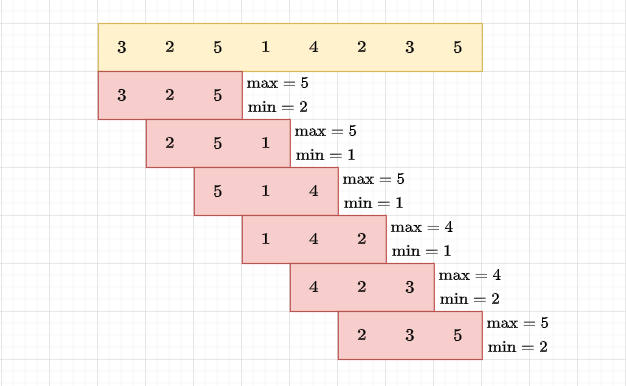
\includegraphics[scale=0.7]{images/sliding_max_min.png}
    \end{center}
\end{frame}

\begin{frame}[fragile]{單調隊列}
    \begin{block}{Sliding Maximum/Minimum (Zerojudge a146)}
        你有一個長度為 $n$ 的陣列 $a_1, \dots, a_n$,請找出所有長度為 $k$ 的子陣列的最大和最小值。 \\
        \vspace{5mm}
        測資範圍: $n \le 10^6$
    \end{block}
    
    我們要怎麼做到這一點呢? 此時,單調隊列可以幫助我們做到這一點!
\end{frame}

\begin{frame}[fragile]{單調隊列}
    現在,我們想一個簡單一點的問題,我們對前綴找出維護最大值的單調隊列試試
    \begin{center}
        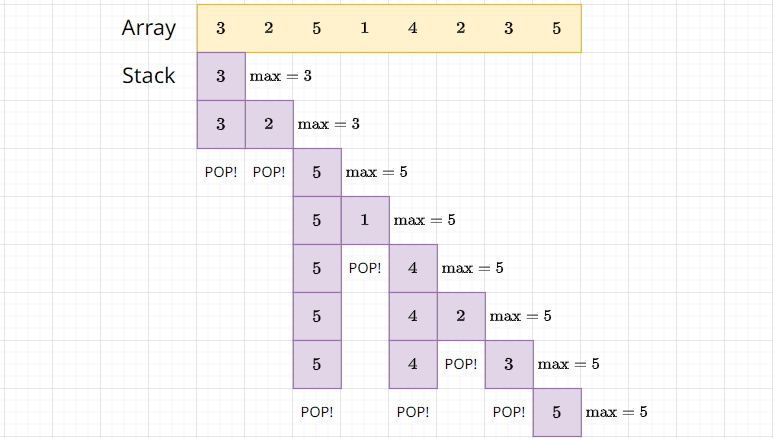
\includegraphics[scale=0.45]{images/prefix_max.png}
    \end{center}
\end{frame}

\begin{frame}[fragile]{單調隊列}
    用一樣的做法,不過長度超過 $k$ 的也跟著 POP 掉!
    \begin{center}
        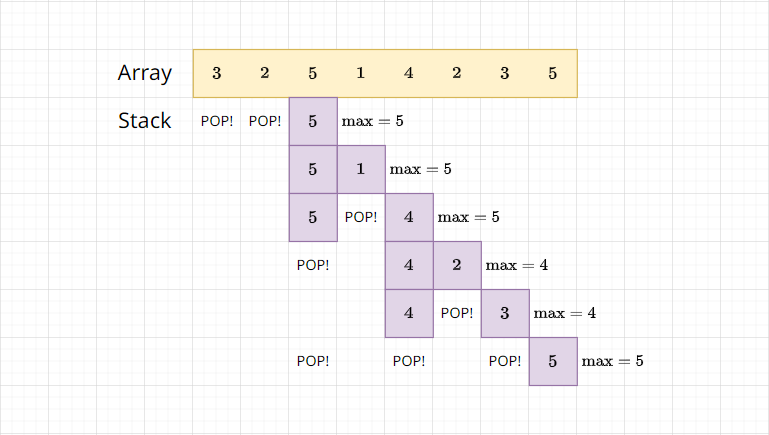
\includegraphics[scale=0.45]{images/sliding_max.png}
    \end{center}
\end{frame}

\begin{frame}[fragile]{單調隊列}
    只要對最大最小值都做一樣的事情,就可以得到固定長度的區間ㄌ。 \\
    時間複雜度: $O(n)$,比直接用 set 等資料結構還要快!
\end{frame}

\begin{frame}[fragile]{單調隊列優化}
    \begin{block}{Zerojudge c528. 相隔小於一定距離最小總和子序列}
    給定一個長度為 $N$ 的整數序列 $a_1,a_2,\dots,a_N$
    及一個正整數 $K$ ,請蓋掉任意個數字使得原序列中任意的連續 $K$ 個數字都至少有一個數字被蓋掉了,請問蓋掉的數字的總和最小為多少?
    \end{block} \pause
    這題的 DP 式大家可以想一下,有想法的都可以提出來。
\end{frame}

\begin{frame}[fragile]{單調隊列優化}
    \begin{block}{Zerojudge c528. 相隔小於一定距離最小總和子序列}
    給定一個長度為 $N$ 的整數序列 $a_1,a_2,\dots,a_N$
    及一個正整數 $K$ ,請蓋掉任意個數字使得原序列中任意的連續 $K$ 個數字都至少有一個數字被蓋掉了,請問蓋掉的數字的總和最小為多少?
    \end{block} 
    設 $dp[i]$ 為遮掉第 $i$ 個元素且前 $i$ 個數字滿足題目條件時的最小總和。 \\
    則轉移式為
        $$dp[i] = \min_{j=\max(0,i-k)}^{i-1}(dp[j]+a[i])$$ \\
    這個轉移式,我們可以很輕易地使用兩個迴圈,在 $O(NK)$ 的時間做完
\end{frame}

\begin{frame}[fragile]{單調隊列優化}
    \begin{block}{Zerojudge c528. 相隔小於一定距離最小總和子序列}
    給定一個長度為 $N$ 的整數序列 $a_1,a_2,\dots,a_N$
    及一個正整數 $K$ ,請蓋掉任意個數字使得原序列中任意的連續 $K$ 個數字都至少有一個數字被蓋掉了,請問蓋掉的數字的總和最小為多少?
    \end{block} 
        $$dp[i] = \min_{j=\max(0,i-k)}^{i-1}(dp[j])+a[i]$$ \\
    不過,觀察到,其實我們只是想要找一段固定長度的區間的最小值! \\
    單調隊列! 時間複雜度: $O(n)$
\end{frame}

\section{矩陣快速冪}

\begin{frame}[fragile]{矩陣乘法!}
    在上禮拜的數學課,不知道大家有沒有把矩陣乘法這個東西學起來呢? \\
    $$A_{n \times m} B_{m \times p} = \sum_{k=1} a_{ik} b_{kj}$$ \\
    
    \begin{center}
        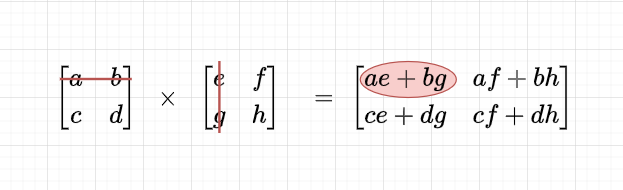
\includegraphics[scale=0.45]{images/matrix multiplication.png}
    \end{center}
\end{frame}

\begin{frame}[fragile]{矩陣乘法!}
    我們可以將矩陣寫成 struct,會像是以下這樣。 乘法時間複雜度為 $O(nmp)$
    
    \begin{center}
        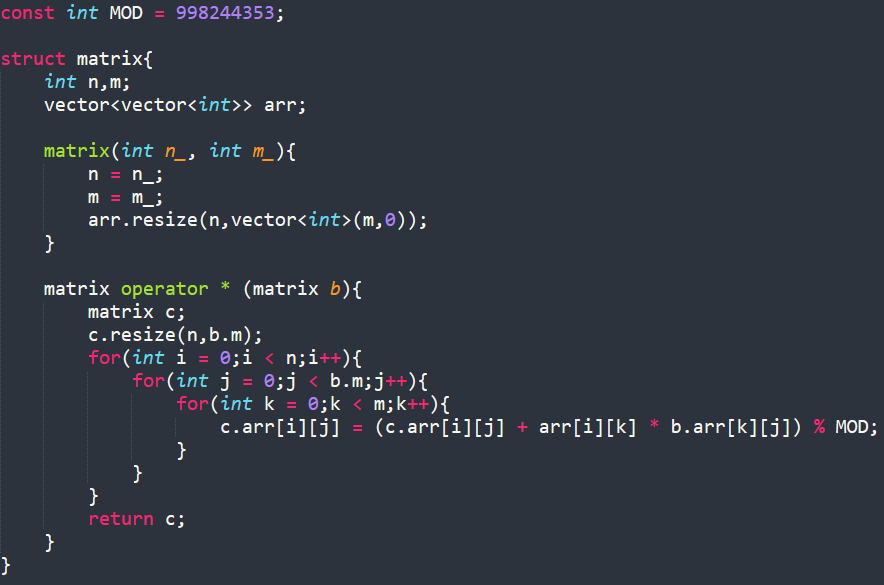
\includegraphics[scale=0.45]{images/matrix.png}
    \end{center}
\end{frame}

\begin{frame}[fragile]{跟 DP 有什麼關係?}
    \begin{block}{費氏數列第 $n$ 項! (CSES - Fibonacci Numbers)}
        費氏數列,是一個定義為以下的數列
        \begin{itemize}
            \item $f_0 = 1$
            \item $f_1 = 1$
            \item $f_n = f_{n-1}+f_{n-2}$
        \end{itemize}
        現在,請找到費氏數列第 $n$ 項 ($n \le 10^{18}$),請輸出 $\mod 10^9+7$ 後的結果
    \end{block}
    $n$ 超級大欸? 該怎麼辦呢?
\end{frame}

\begin{frame}[fragile]{跟 DP 有什麼關係?}
    \begin{block}{費氏數列第 $n$ 項! (CSES - Fibonacci Numbers)}
        費氏數列,是一個定義為以下的數列
        \begin{itemize}
            \item $f_0 = 1$
            \item $f_1 = 1$
            \item $f_n = f_{n-1}+f_{n-2}$
        \end{itemize}
        現在,請找到費氏數列第 $n$ 項 ($n \le 10^{18}$),請輸出 $\mod 10^9+7$ 後的結果
    \end{block}
    我們將轉移式寫成矩陣!
    $$\begin{bmatrix}f_{n} \\ f_{n-1} \end{bmatrix} = \begin{bmatrix}1 & 1 \\ 1 & 0 \end{bmatrix} \begin{bmatrix}f_{n-1} \\ f_{n-2} \end{bmatrix}$$
\end{frame}

\begin{frame}[fragile]{跟 DP 有什麼關係?}
    \begin{block}{費氏數列第 $n$ 項! (CSES - Fibonacci Numbers)}
        費氏數列,是一個定義為以下的數列
        \begin{itemize}
            \item $f_0 = 1$
            \item $f_1 = 1$
            \item $f_n = f_{n-1}+f_{n-2}$
        \end{itemize}
        現在,請找到費氏數列第 $n$ 項 ($n \le 10^{18}$),請輸出 $\mod 10^9+7$ 後的結果
    \end{block}
    轉換一下!
    $$\begin{bmatrix}f_{n} \\ f_{n-1} \end{bmatrix} = \begin{bmatrix}1 & 1 \\ 1 & 0 \end{bmatrix}^{n-1} \begin{bmatrix}f_1 \\ f_0 \end{bmatrix}$$
\end{frame}

\begin{frame}[fragile]{跟 DP 有什麼關係?}
    \begin{block}{費氏數列第 $n$ 項! (CSES - Fibonacci Numbers)}
        費氏數列,是一個定義為以下的數列
        \begin{itemize}
            \item $f_0 = 1$
            \item $f_1 = 1$
            \item $f_n = f_{n-1}+f_{n-2}$
        \end{itemize}
        現在,請找到費氏數列第 $n$ 項 ($n \le 10^{18}$),請輸出 $\mod 10^9+7$ 後的結果
    \end{block}
    出現了次方,有什麼東西可以幫我們做次方的動作呢? \pause
    快速冪!
\end{frame}


\begin{frame}[fragile]{矩陣快速冪}
    因此,我們將快速冪寫成矩陣的版本
    \begin{center}
        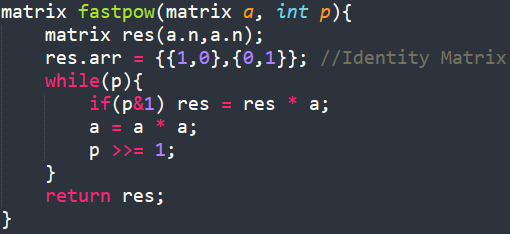
\includegraphics[scale=0.7]{images/matrix_exponentiation.png}
    \end{center}
\end{frame}

\begin{frame}[fragile]{矩陣快速冪}
    \begin{block}{費氏數列第 $n$ 項! (CSES - Fibonacci Numbers)}
        費氏數列,是一個定義為以下的數列
        \begin{itemize}
            \item $f_0 = 1$
            \item $f_1 = 1$
            \item $f_n = f_{n-1}+f_{n-2}$
        \end{itemize}
        現在,請找到費氏數列第 $n$ 項 ($n \le 10^{18}$),請輸出 $\mod 10^9+7$ 後的結果
    \end{block}
    我們就可以在 $O(2^3 \log n)$ 的時間找到費氏數列第 $n$ 項了!
\end{frame}

\begin{frame}[fragile]{矩陣快速冪可以使用的地方?}
    一定有人很好奇,既然費氏數列可以用這樣的方式計算,那還有哪些 DP 也能這樣做呢? \\ \pause
    可以使用矩陣快速冪的 DP,通常會出現一種「線性遞迴」的形式 
    \begin{alertblock}{線性遞迴}
        每一項與前幾項的關係都是線性的!
        $$dp_i = a_1 dp_{i-1} + a_2 dp_{i-2} + \cdots $$
    \end{alertblock}
\end{frame}

\begin{frame}[fragile]{例題}
    \begin{block}{骰骰子問題 EX (CSES - Throwing Dice)}
        你有一顆六面的骰子,每個骰子可以骰出 $1 \sim 6$ 點。請問你總共有幾種方式經由骰很多次骰子湊出 $x$ 點。 ($x \le 10^{18}$)
    \end{block} \pause
    這題上週 Colten 在 DP I 的課講過了一模一樣的例題,不過,範圍變大了? \pause
    原本的轉移式是
        $$dp_i = dp_{i-1} + dp_{i-2} + \dots + dp_{i-6}$$ \pause
    事實上,這個就是一個線性遞迴的例子!
\end{frame}

\begin{frame}[fragile]{例題}
    我們可以將其寫成矩陣!
    
    $$\begin{bmatrix} 1 & 1 & 1 & 1 & 1 & 1 \\
                      0 & 1 & 0 & 0 & 0 & 0 \\
                      0 & 0 & 1 & 0 & 0 & 0 \\
                      0 & 0 & 0 & 1 & 0 & 0 \\
                      0 & 0 & 0 & 0 & 1 & 0 \\
                      0 & 0 & 0 & 0 & 0 & 1
    \end{bmatrix} 
    \begin{bmatrix}   dp_{i-1} \\
                      dp_{i-2} \\
                      dp_{i-3} \\
                      dp_{i-4} \\
                      dp_{i-5} \\
                      dp_{i-6}
    \end{bmatrix}$$
\end{frame}

\begin{frame}[fragile]{例題}
    \begin{block}{骰骰子問題 EX (CSES - Throwing Dice)}
        你有一顆六面的骰子,每個骰子可以骰出 $1 \sim 6$ 點。請問你總共有幾種方式經由骰很多次骰子湊出 $x$ 點。 ($x \le 10^{18}$)
    \end{block} 
    因此,這題就可以在 $O(6^3 \log x)$ 的時間完成了!
\end{frame}

\begin{frame}[fragile]{有向圖的矩陣快速冪!}
    在上週,Koying 有教過大家不同的存圖方式,而其中一種,就是「鄰接矩陣」 \\
    由於需要佔據 $n \times n$ 的空間,存取也不會很快,因此我們比較少用 \\
    但是,他其實有個很好的性質!
\end{frame}

\begin{frame}[fragile]{有向圖的矩陣快速冪!}
    \begin{block}{Atcoder DP Contest R - Walk}
        你有一個 $n$ 個節點的有向圖,以及他的鄰接矩陣。請找到這張圖共有幾個長度為 $k$ 的有向路徑。\\ 
        \vspace{5mm}
        測資範圍: $n \le 2000, k \le 10^{18}$
    \end{block}
    這個問題,同樣的,我們可以列出他的 DP 狀態與轉移式 \pause
    設 $dp[i][j][k]$ 表示總共有幾個長度為 $k$ 的路徑,可以從 $i$ 走到 $j$ \\
    轉移式則是 
        $$dp[i][j][k] = \sum_{i \rightarrow l \rightarrow j}(dp[i][l][k-1] \times dp[l][j][1])$$
\end{frame}

\begin{frame}[fragile]{有向圖的矩陣快速冪!}
    \begin{block}{Atcoder DP Contest R - Walk}
        你有一個 $n$ 個節點的有向圖,以及他的鄰接矩陣。請找到這張圖共有幾個長度為 $k$ 的有向路徑。\\ 
        \vspace{5mm}
        測資範圍: $n \le 2000, k \le 10^{18}$
    \end{block}
    我們將轉移式進行滾動! 會得到
        $$dp_k[i][j]= \sum_{j=1}^n(dp_k-1[i][l] \times A[l][j])$$ \\
    他其實是一個線性遞迴!
\end{frame}

\begin{frame}[fragile]{有向圖的矩陣快速冪!}
    \begin{block}{Atcoder DP Contest R - Walk}
        你有一個 $n$ 個節點的有向圖,以及他的鄰接矩陣。請找到這張圖共有幾個長度為 $k$ 的有向路徑。\\ 
        \vspace{5mm}
        測資範圍: $n \le 2000, k \le 10^{18}$
    \end{block}
    而事實上,如果一個陣列的鄰接矩陣是 $A$,則 $A^k_{ij}$ 表示從 $i$ 走到 $j$ 有幾個長度為 $k$ 的有向路徑,因此直接做矩陣快速冪即可!
\end{frame}

\section{更多例題}

\begin{frame}{例題}
    \begin{block}{AtCoder Beginner Contest 237 F - |LIS| = 3}
        給你兩個正整數 $n,m$,請找到有幾個陣列滿足 (LIS 是嚴格遞增的)
        \begin{itemize}
            \item 陣列長度為 $n$
            \item 所有數字介於 $1$ 到 $m$
            \item 陣列的 LIS 為 $3$
        \end{itemize} \\ 
        \vspace{5mm}
        測資範圍: $3 \le n \le 1000, 1 \le m \le 10$
    \end{block} \pause
    這題給大家一點時間思考看看,看看有沒有人有什麼想法。
\end{frame}

\begin{frame}{例題}
    \begin{block}{AtCoder Beginner Contest 237 F - |LIS| = 3}
        給你兩個正整數 $n,m$,請找到有幾個陣列滿足 (LIS 是嚴格遞增的)
        \begin{itemize}
            \item 陣列長度為 $n$
            \item 所有數字介於 $1$ 到 $m$
            \item 陣列的 LIS 為 $3$
        \end{itemize} \\ 
        \vspace{5mm}
        測資範圍: $3 \le n \le 1000, 1 \le m \le 10$
    \end{block} 
    設 $dp[i][a][b][c]$ 表示有幾個陣列長度為 $i$,且 LIS 的 $v$ 陣列為 $\{a,b,c\}$ 
\end{frame}

\begin{frame}[fragile]{例題}
    實作如下
    \begin{center}
        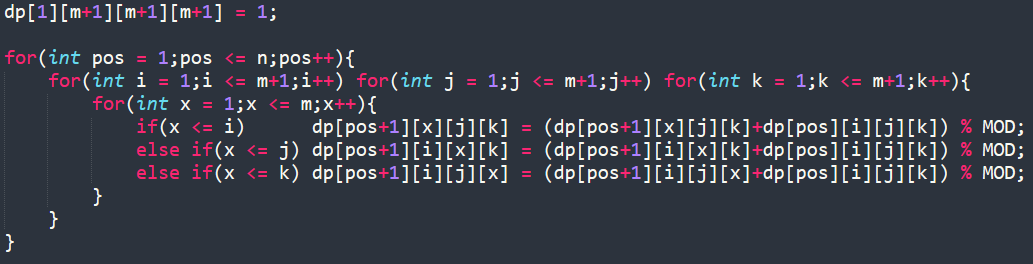
\includegraphics[scale=0.5]{images/LIS is three.png}
    \end{center}
\end{frame}

\begin{frame}{例題}
    \begin{block}{Codeforces 895C - Square Subsets}
        現在,你有長度為 $n$ 的陣列 $a_1,a_2,\dots,a_n$,請找到陣列中有幾個相異的非空子集,其中的元素的乘積為完全平方數\\ 
        \vspace{5mm}
        測資範圍: $3 \le 10^5, 1 \le a_i \le 70$
    \end{block} \pause
    這題同樣給大家一點時間想想看
\end{frame}

\begin{frame}{例題}
    \begin{block}{Codeforces 895C - Square Subsets}
        現在,你有長度為 $n$ 的陣列 $a_1,a_2,\dots,a_n$,請找到陣列中有幾個相異的非空子集,其中的元素的乘積為完全平方數\\ 
        \vspace{5mm}
        測資範圍: $3 \le 10^5, 1 \le a_i \le 70$
    \end{block} 
    首先,觀察到數字最大只有到 $70$,小於 $70$ 的質數一共只有 $18$ 個! \\
    另外一點是,如果要是完全平方數,所有質因數的次方必須是 $2$ 的倍數! \\
    我們用 bitmask 中第 $i$ 位的 $0/1$ 表示質因數的次方是偶數還是奇數。
\end{frame}

\begin{frame}{例題}
    \begin{block}{Codeforces 895C - Square Subsets}
        現在,你有長度為 $n$ 的陣列 $a_1,a_2,\dots,a_n$,請找到陣列中有幾個相異的非空子集,其中的元素的乘積為完全平方數\\ 
        \vspace{5mm}
        測資範圍: $3 \le 10^5, 1 \le a_i \le 70$
    \end{block} 
    設 $dp[mask]$ 表示有幾種集合的數字乘積為 $mask$,答案就會是 $dp[0] - 1$ 了 \\
    分別枚舉 $1 \sim 70$ 每個數字要不要拿,進行轉移即可
\end{frame}

\begin{frame}[fragile]{例題}
    實作如下:
    \begin{lstlisting}[language=C++]
dp[0][0] = 1;
for(int i = 1;i <= 70;i++){
    for(int j = 0;j < (1<<18);j++){
        if(!cnt[i]) dp[i][j] = dp[i-1][j];
    else dp[i][j] = (dp[i][j] + dp[i-1][j] + dp[i-1][j^num[i]])%MOD * fastpow(2,cnt[i]-1)%MOD;
    }
}
    \end{lstlisting}
\end{frame}

\section{補充}

\begin{frame}{輪廓線 DP}
    \begin{center}
        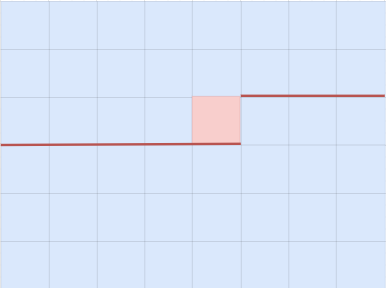
\includegraphics[scale=0.8]{images/DP on Broken Profile.png}
    \end{center}
\end{frame}


\end{document}